\chapter{Materials and Methods}\label{chap:methods}


Before walking through the workflow stages one by one, an overview of the whole is worth a glance: Figures~\ref{fig:overview} and~\ref{fig:overview-r} split it into two halves by the one artifact they share---an unfiltered isoform count matrix. The first half turns raw \gls{fastq} reads into transcript-level counts (Section~\ref{sec:pipeline}); the second takes that matrix, filters and cleans it, and runs the COTAN analysis and turns the counts into \gls{dtu} candidates (Sections~\ref{sec:data-filtering} and \ref{sec:methods-dtu-algorithm} onward).

Each half is implemented by a separate piece of code. The first half is driven by a custom Nextflow pipeline written for this thesis: it chains download, index, alignment and quantification around \texttt{nf-core/scrnaseq} (v4.1.0), runs on the cluster, and ends where the raw count matrix is written. The second half is driven by the \texttt{cotanisoform} R package together with config-driven analysis scripts, both written for this thesis; they consume that matrix, filter and clean it, and run COTAN to yield the \gls{dtu} candidates. The two halves therefore never share a runtime: the heavy sequencing work lives in Nextflow, the statistical work in R.


\usetikzlibrary{arrows.meta, positioning, decorations.pathreplacing}
\begingroup
\setlength{\textfloatsep}{2em plus 2pt minus 4pt}
\setlength{\floatsep}{1em plus 2pt minus 2pt}
\vspace{2em}
\begin{figure}[htbp]
    \centering
    \resizebox{\linewidth}{!}{%
    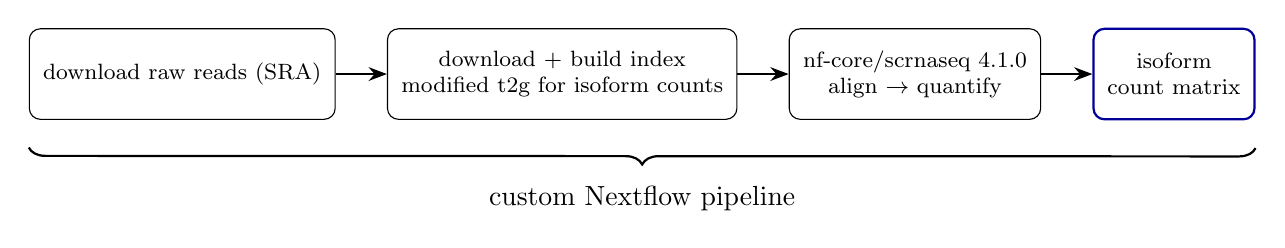
\begin{tikzpicture}[
        box/.style={draw, rounded corners, minimum height=1.15cm, inner sep=5pt, align=center, font=\footnotesize},
        arr/.style={-{Stealth}, thick},
        sep/.style={right=0.65cm of #1},
    ]
        \node[box] (reads) at (0,0) {download raw reads (SRA)};
        \node[box, sep=reads] (index) {download + build index\\modified t2g for isoform counts};
        \node[box, sep=index] (quant) {nf-core/scrnaseq 4.1.0\\align $\rightarrow$ quantify};
        \node[box, draw=blue!60!black, thick, sep=quant] (matrix) {isoform\\count matrix};

        \draw[arr] (reads) -- (index);
        \draw[arr] (index) -- (quant);
        \draw[arr] (quant) -- (matrix);

        \draw[thick, decorate, decoration={brace, amplitude=6pt, mirror}]
            ([yshift=-10pt]reads.south west) -- ([yshift=-10pt]matrix.south east)
            node[midway, below=10pt] {custom Nextflow pipeline};
    \end{tikzpicture}}
    \caption{Overview of the first half of the workflow: a custom Nextflow pipeline turns raw \gls{fastq} reads into an unfiltered isoform count matrix.}
    \label{fig:overview}
\end{figure}

\begin{figure}[htbp]
    \centering
    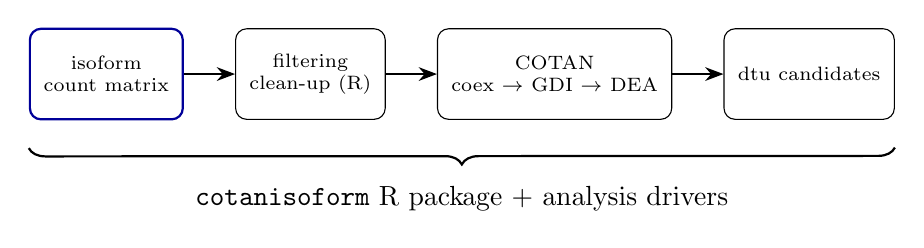
\begin{tikzpicture}[
        box/.style={draw, rounded corners, minimum height=1.15cm, inner sep=5pt, align=center, font=\scriptsize},
        arr/.style={{-{Stealth}}, thick},
        sep/.style={right=0.65cm of #1},
    ]
        \node[box, draw=blue!60!black, thick] (matrix) {isoform\\count matrix};
        \node[box, sep=matrix] (filter) {filtering\\clean-up (R)};
        \node[box, sep=filter] (cotan) {COTAN\\coex $\rightarrow$ GDI $\rightarrow$ DEA};
        \node[box, sep=cotan] (dtu) {\gls{dtu} candidates};

        \draw[arr] (matrix) -- (filter);
        \draw[arr] (filter) -- (cotan);
        \draw[arr] (cotan) -- (dtu);

        \draw[thick, decorate, decoration={brace, amplitude=6pt, mirror}]
            ([yshift=-10pt]matrix.south west) -- ([yshift=-10pt]dtu.south east)
            node[midway, below=10pt] {\texttt{cotanisoform} R package + analysis drivers};
    \end{tikzpicture}
    \caption{Overview of the second half of the workflow: the isoform count matrix is filtered, cleaned, and processed through COTAN's co-expression, GDI and DEA stages to yield the \gls{dtu} candidates.}
    \label{fig:overview-r}
\end{figure}
\endgroup

Table~\ref{tab:toolchain} records the tools and versions used in both halves, each with the section that justifies its choice.

\begin{table}[htbp]
    \caption{Tools used in this thesis: role, version, and the section justifying each choice.}\label{tab:toolchain}
    \vspace{0.5em}
    \small
    \setlength{\tabcolsep}{5pt}
    \begin{tabular}{@{}l l >{\raggedright\arraybackslash}p{8.5em} l@{}}
        \toprule
        \textbf{Tool} & \textbf{Version} & \textbf{Role} & \textbf{Justified in} \\
        \midrule
        Nextflow & 26.04.4 & Pipeline orchestration & \ref{sec:pipeline} \\
        nf-core/scrnaseq & 4.1.0 & Automates index $\rightarrow$ align $\rightarrow$ quantify & \ref{sec:pipeline} \\
        simpleaf & 0.24.1 quant.\,/\,0.24.0 index & Orchestrates alevin-fry + piscem & \ref{sec:pipeline} \\
        alevin-fry & --- & Quantification; EM assignment & \ref{sec:pipeline} \\
        piscem & --- & Index construction & \ref{sec:pipeline} \\
        sra-tools & --- & FASTQ download & \ref{sec:pipeline} \\
        Ensembl & release 102 & Reference annotation & \ref{sec:pipeline} \\
        R & 4.5.3 & Analysis layer & \ref{sec:data-filtering} \\
        COTAN & 2.13.1 (be93aa8) & Contingency, co-expression, DEA, DTU & \ref{sec:data-filtering} \\
        Seurat & 5.5.1 & Count-object container & \ref{sec:data-filtering} \\
        \bottomrule
    \end{tabular}
\end{table}

\section{Data Acquisition and Dataset Selection}

This study is based on two publicly available, droplet-based single-cell RNA-sequencing datasets: the Arigoni human cell-line mixture (GSE243665\cite{arigoni2024benchmark}) and the Ding mouse brain dataset (GSE132044\cite{ding2020systematic}). Both were obtained as raw \gls{fastq} reads alongside their genome annotations. They were selected after evaluating potential candidates against specific inclusion criteria, which are detailed below.

Candidate datasets were drawn from the curated collection at \url{https://seriph78.github.io/COTAN_Datasets_analysis/}, rather than searching the Gene Expression Omnibus (GEO)\defn{Gene Expression Omnibus (GEO)}{NCBI's public database of published gene-expression datasets. It stores raw and processed data for re-analysis.}\cite{barrett2013geo} ad hoc. Importantly, these datasets are pre-validated. Their prior use in COTAN's original benchmarking studies confirms their compatibility with the framework and ensures they are free of major technical artifacts.

A limitation of this collection is the absence of publicly available transcript-level count matrices for \gls{scRnaSeq} data. This reflects standard field practices rather than an omission. By default, most pipelines---including CellRanger\defn{CellRanger / Seurat}{Standard pipelines (10x CellRanger, Seurat) that quantify and analyse scRNA-seq data, defaulting to gene-level counts.}\cite{zheng2017massively} and the standard Seurat workflow\cite{hao2024seurat}---collapse data to \gls{gene}-level counts. While transcript quantification is possible using pseudo-alignment tools like Salmon\cite{patro2017salmon} or alevin-fry\cite{he2022alevin}, these steps are frequently bypassed. Furthermore, even when transcript-level analysis is performed, the data is typically aggregated back to the gene level prior to publication. Consequently, transcript matrices must be generated directly from the raw \gls{fastq} files.

That rebuild can be automated from scratch with the \texttt{nf-core/scrnaseq} pipeline\cite{ewels2020nfcore}, a containerised Nextflow workflow that chains indexing, alignment and quantification behind a single invocation.

That choice, however, narrows the field: \texttt{nf-core/scrnaseq} supports barcode-based protocols only, with the 10x Genomics\cite{zheng2017massively} chemistries, versions 2 and 3, as the supported family, so any dataset analysed here must come from that chemistry family. Of the COTAN datasets, only the Arigoni human cell-line mixture and the Ding mouse brain dataset satisfy both this chemistry requirement and the availability of published barcode lists --- the two datasets introduced above.

Those two are, in fact, a fortunate pairing. The Arigoni mixture is the strong-signal case: its cell lines are well separated and each carries a distinct isoform programme, and its GEO deposit supplies published barcode labels per line, so the detector runs against known groups and its calls can be checked against cell-type identity. The Ding cortex is the weak-signal case: heterogeneous tissue with gradual transitions and subtler contrasts, where no published labels exist, so it forces the computational-partitioning route and the cross-resolution validation. The pair therefore brackets the difficulty spectrum---a clean, discrete test and a noisy, continuous one---so that the candidates converging across both (Chapter~\ref{chap:results}) argue for a method that generalises rather than one fitted to a single favourable context.

\subsection*{Raw Read Download}\label{sec:download}

The raw input is not uniformly FASTQ. SRA stores 10x single-read runs as aligned BAM files rather than as reads, so the download path depends on each accession's layout. A layout check picks the route: paired-end runs are fetched as FASTQs via \texttt{prefetch} + \texttt{fasterq-dump}, whereas single-end 10x runs are fetched as the TenX BAM (\texttt{prefetch --type TenX}) and converted back to FASTQs with \texttt{bamtofastq}\cite{leinonen2011sra}. The Arigoni and Ding deposits are both 10x single-end runs, so both take the BAM-then-\texttt{bamtofastq} path.

Two operational choices keep the downloads tractable. They stage in RAM (\texttt{/dev/shm}) and never touch persistent disk, because each sample is tens of gigabytes---about 18~GB of BAM or 8~GB of zipped FASTQ. And concurrency is capped to stay within SRA's rate limits.

\section{Alignment, Quantification, and Feature Generation}\label{sec:pipeline}

\subsection*{Algorithm Selection: alevin-fry (simpleaf) vs.\ kallisto}

Quantifying transcripts from raw reads requires a choice between alignment-based and pseudo-alignment-based pipelines, and that choice propagates into the UMI handling and ambiguity resolution that downstream analysis depends on. Pseudo-alignment was preferred here for the reasons set out in Section~\ref{sec:pseudo-align}. Two pseudo-aligners dominate single-cell transcript quantification, each pairing a pseudo-alignment engine with a UMI-deduplication step: kallisto with bustools, and alevin-fry with its \texttt{simpleaf} orchestrator. Table~\ref{tab:pseudoalign-tools} compares their primary characteristics.

\begin{table}[htbp]
    \centering
    \caption{Comparison of scRNA-seq pseudo-alignment architectures.}\label{tab:pseudoalign-tools}
    \vspace{0.5em}
    \small
    \setlength{\tabcolsep}{6pt}
    \resizebox{\linewidth}{!}{%
    \begin{tabular}{lcc}
        \toprule
        \textbf{Feature} & \textbf{kallisto | bustools} & \textbf{alevin-fry (simpleaf)} \\
        \midrule
        Multi-mapping handling & Full compatible set & Minimal set (parsimony) \\
        \gls{umi} deduplication & Standard collapse & Directional error modelling \\
        Execution speed & Fast ($\sim$10 min per sample) & Very fast ($\sim$5 min per sample) \\
        nf-core integration & Available, non-standard & Native (v4.1.0) \\
        \bottomrule
    \end{tabular}}
\end{table}

The \texttt{simpleaf} framework\cite{he2023simpleaf} (v0.24.1 for quantification, v0.24.0 for the index build), which orchestrates \texttt{alevin-fry} for quantification and \texttt{piscem} for indexing, was selected for three reasons. Its UMI handling is superior, since single-cell data relies on \glspl{umi} to correct \gls{pcr} amplification bias and the alevin-fry error model distinguishes true UMIs from sequencing errors more reliably. For reads compatible with multiple transcripts, alevin-fry resolves the ambiguity by parsimony, searching for the minimal set of transcripts that explains each UMI rather than counting it against every compatible transcript, which suppresses spurious low-abundance counts that would bias the within-gene proportions that \gls{dtu} detection reads out. Finally, \defn{nf-core}{A community repository of standardised, peer-reviewed Nextflow analysis pipelines.}nf-core/scrnaseq (v4.1.0) supports \texttt{simpleaf} natively, with fewer configuration quirks than the kallisto alternatives.

The parsimony resolution matters. Assigning a UMI to the full set of transcripts it is compatible with leaks counts from an abundant isoform onto lowly-expressed isoforms sharing its sequence, biasing the within-gene proportions that \gls{dtu} detection reads out. \texttt{parsimony}\defn{parsimony}{An alevin-fry \gls{umi}-resolution mode that searches for the minimal set of transcripts explaining each UMI, suppressing spurious low-abundance counts.} instead builds a parsimony graph and finds the minimal set of transcripts that explains each UMI, so spurious low-abundance counts are suppressed and the estimated proportions are better identified. The resolution can leave fractional counts on ties, which are rounded to integers before COTAN ingests the matrix.

Because the downstream analysis operates on binary presence and absence rather than on the abundance point estimates, bootstrapped abundance variance was not part of this pipeline and is of limited relevance to zero-based detection: the rounded counts are discretised into detection indicators before the co-expression statistics are computed.

\subsection*{Index Modification for Transcript-Level Resolution}\label{sec:modification-process}

Standard alevin-fry\cite{he2022alevin} output collapses to gene level by default via transcript-to-gene mapping\defn{Transcript-to-gene (t2g) mapping}{A file pairing each transcript with its parent gene; replacing it with an identity mapping prevents gene-level collapse.}. To extract transcript counts, the index files were modified before alignment, following the identity-mapping route discussed in the \texttt{simpleaf} issue tracker\footnote{\url{https://github.com/COMBINE-lab/simpleaf/issues/115} (accessed 29 September 2026)}:

\begin{enumerate}
    \item \textbf{Identity mapping in \texttt{t2g\_3col.tsv}}: the standard mapping is replaced by a self-referential one, which prevents the final aggregation step that sums isoforms into genes.
{\small\begin{verbatim}
# Original: ENSMUST00000193814  ENSMUSG00000067548  # parent gene
# Modified: ENSMUST00000193814  ENSMUST00000193814  # itself
\end{verbatim}}

    \item \textbf{Removal of \texttt{gene\_id\_to\_name.tsv}}: the nf-core pipeline uses this file to map Ensembl gene identifiers to gene names during annotation. With the identity mapping in place the matrix rows are Ensembl \emph{transcript} identifiers, so the annotation step finds no gene IDs to match and halts. Removing \texttt{gene\_id\_to\_name.tsv} from the index trips a safety guard in alevin-fry: the annotation step checks for the file's presence and, finding it absent, skips the step. The guard does not itself know that annotation would halt on transcript IDs; the removal is deliberate, and it prevents that halt. The transcript counts were already written to disk, so they are kept and carried into the analysis.
\end{enumerate}

This modification is \textbf{reversible}: transcript-level quantification is a finer partition of the gene-level signal, so summing the transcript rows by gene using the retained \texttt{t2g} and \texttt{gene\_id\_to\_name} tables recovers a gene-level matrix directly, without rebuilding the index or re-aligning. This transcript-level route is an unsupported workaround, since alevin-fry is built for gene-level collapse and the identity-mapping modification is not an official mode. The gene-level matrix recovered by summing the transcript rows therefore matches a native gene-level run, except where the two resolutions assign ambiguous reads differently.

\subsection*{Reproducible Workflow Automation}

To make this workflow reproducible across datasets, it was automated with \textbf{Nextflow}\cite{ditommaso2017nextflow} (v26.04.4), a domain-specific language for computational pipelines that handles parallelization and checkpointing. This choice provides error handling, containerized dependencies, and standard configuration across datasets.

The custom automation script:

\begin{itemize}
    \item \textbf{Input}: a CSV samplesheet listing each sample and its SRA accessions\defn{Sequence Read Archive (SRA)}{NCBI's repository of raw sequencing data, accessed by identifiers such as SRR accessions.}, and a per-dataset configuration naming the genome assembly and species, the Ensembl release (102), the 10x chemistry, and the published barcode list. The pipeline downloads the reference FASTA and GTF\defn{GTF (Gene Transfer Format)}{An annotation file listing each gene's coordinates, exon structure, and transcript boundaries; used to build the transcriptome index.} from Ensembl itself, so a matching assembly name replaces a manual reference download. The configuration is not limited to these fields: it also carries options for the alignment mode, the index strategy, and other pipeline parameters, which are left at sensible defaults unless a dataset needs them.
    \item \textbf{Automated steps}:
    \begin{enumerate}
        \item Download the raw reads (Section~\ref{sec:download}): FASTQs for paired-end runs, BAM-then-\texttt{bamtofastq} for 10x single-end runs.
        \item Download the Ensembl reference and build the gene-level \texttt{piscem} index.
        \item If transcript-level output is requested, create a cheated transcript-level copy of that index by applying the identity-mapping modification.
        \item Execute nf-core/scrnaseq (v4.1.0) with \texttt{simpleaf}.
        \item Produce the raw count matrix and its metadata.
    \end{enumerate}
    \item \textbf{Availability}: the complete workflow, including configuration files and test cases, is available at \url{https://github.com/ldelitala/sc-isoform-cotan}.
\end{itemize}

The workflow ends at the count matrix. Quality filtering and the COTAN analysis are performed afterwards in the R analysis layer (R 4.5.3), keeping the two concerns separate.

Adapter trimming is omitted deliberately rather than by oversight. The 10x read structure places the barcode and UMI in a fixed header segment, and \texttt{simpleaf} resolves that geometry internally with a UMI-aware error model, discarding residual adapter $k$-mers because they match no indexed sequence. A separate \texttt{fastp} pass would therefore reread the entire FASTQ file for no change in the count matrix. Quality control at the barcode level still runs: \texttt{simpleaf} applies empty-droplet detection to the quantification output, and cells are further restricted to the high-quality barcode sets published with each dataset (Section~\ref{sec:data-filtering}).

\section{Data Processing and Quality Control}\label{sec:data-filtering}

Before the COTAN object is built, the Seurat assay's counts are rounded to the nearest integer and explicit zeros are dropped, since COTAN ingests integer counts; the fractional parsimony-em assignments never enter the framework directly. The COTAN object is then initialised from this Seurat object, and all subsequent filtering operates on it. From this point onward Seurat is no longer used; the rest of the workflow operates exclusively on the COTAN object.

\subsection*{Cell-Level Filtering}

Cells were filtered using metadata from the original GEO publications. The Arigoni dataset (GSE243665\cite{arigoni2024benchmark}) and the Ding dataset (GSE132044\cite{ding2020systematic}) both provide lists of cells that passed their quality control thresholds, and restricting the analysis to those known-good barcodes avoids a second QC pipeline that could introduce inconsistencies. Published studies typically filter on a minimum UMI count per cell, which removes empty droplets; a maximum mitochondrial read percentage\defn{Mitochondrial read percentage}{The fraction of a cell's reads coming from mitochondrial genes; abnormally high values flag dying or damaged cells.}, which removes dying cells; and a gene detection threshold, since cells with too few detected genes may be doublets or otherwise low quality. Reusing their filtering ensures comparability and reduces methodological drift.

The unfiltered matrices are dominated by empty droplets; restricting to the barcodes the original studies report as passing their quality control yields the cell counts. Concretely, the passing-cell barcode lists were loaded into the COTAN object as a \texttt{passed\_QC} condition using the package's \texttt{flag\_valid\_cells\_from\-\_tsv()}, and the object was then subset with \texttt{filter\_cotan\_by\-\_condition()} to keep only cells flagged as passing; the per-cell-line Arigoni lists were combined first. Both functions are part of the \texttt{cotanisoform} R package\cite{ldelitala2026scisoform}, built on top of COTAN's object model.

\subsection*{Feature-Level Filtering}

Feature filtering ran in the R analysis layer (R 4.5.3) with COTAN (v2.13.1, commit \texttt{be93aa8}). Two filters act on the transcript set. First, \texttt{filter\_spliced\_transcripts()} keeps only spliced transcripts by matching the Ensembl feature names against a prefix (\textasciicircum\texttt{ENST} for human, \textasciicircum\texttt{ENSMUST} for mouse) and discarding the rest, then drops the cells that are left with no surviving feature. COTAN's framework\cite{galfre2021cotan} targets mature mRNA, and unspliced pre-mRNA has different statistical properties that can confound \gls{coexpression} analysis, so this restriction to spliced features both removes noise and shrinks the matrix. Second, \texttt{clean\_cotan\_data()} wraps COTAN's \texttt{clean()} routine with its default cutoffs: a transcript is kept only if it is expressed in at least 0.3\% of cells (\texttt{cellsCutoff}=0.003) and a cell only if it detects at least 0.2\% of the retained features (\texttt{genesCutoff}=0.002)---fractional cutoffs far stricter than a fixed count, because isoform-level detection is so sparse that an absolute threshold would admit thousands of near-empty rows. With \texttt{drop\_fully\_expressed} enabled, the few transcripts expressed in nearly every cell are physically removed as well.

These choices prioritize quality over quantity. Smaller matrices mean faster computation and cleaner signal---important when running expensive contingency table calculations across all feature pairs.

\subsection*{Statistical Estimation and the GDI}

With the filtered transcript matrix in the COTAN object, the framework's parameters are estimated and its statistics computed. The per-feature and per-cell expression probabilities $\lambda$ and $\nu$ are calibrated from the observed zeros, the pairwise co-expression coefficient $C_{f,f'}$ and its $p$-value are calculated for every feature pair, and the \gls{gdi} is derived from those $p$-values as the per-feature mean of the smallest $5\%$---the theory is laid out in Section~\ref{sec:cotan-framework}. The pipeline executes all of this in one step (\texttt{03\_calc.R}) and renders the resulting GDI into a diagnostic plot (\texttt{04\_gdi.R}) over a dataset-specific marker panel. This is the stage that turns the filtered counts into the co-expression structure the partition in the next section reads out of; without it, clustering would have nothing to group cells by.

\section{Population Partitioning and Validation}

Differential transcript usage is a contrast between groups of cells: an isoform switch surfaces only when the cells carrying one variant can be set against the cells carrying the other. The partition of cells fixes what the detector is able to see, and the two datasets reach that partition along different routes.

\subsection*{Ground-Truth vs.\ Computational Partitioning}

The Arigoni human cell-line dataset arrives already divided: its GEO deposit distributes one barcode list per constituent cell line and for the PBMCs, so those published labels serve directly as the groups the detector compares.

The Ding mouse cortex dataset arrives with no such labels. Its cells are grouped from the matrix itself with COTAN's hierarchical uniform clustering\defn{Hierarchical uniform clustering}{COTAN's procedure that recursively splits cells by co-expression dissimilarity, then merges statistically indistinguishable clusters.}. Cell-to-cell dissimilarity is read from the co-expression patterns, clusters are split until each becomes homogeneous, and neighbours the statistics cannot separate are merged. Run on transcript counts, the procedure returns a set of uniform clusters and a small noisy remainder---the cells whose expression matches no group closely enough to claim them. Those clusters are a hypothesis, not a verdict: COTAN was designed and validated on gene-level matrices, and this thesis is its first application at isoform level, so nothing guarantees the co-expression statistics still hold on transcripts.

\subsection*{Cross-Resolution Validation}

To give the transcript partition something to be measured against, the same cells were clustered a second time on gene counts: the official Ding gene matrix, cleaned with COTAN's standard \texttt{clean()} and clustered with parameters identical to the transcript run. Gene-level clustering is the established use of COTAN; over a denser feature set it stands as an independent reference partition rather than a cheaper substitute. The two partitions are then compared over their common cells by a confusion matrix\defn{Confusion matrix}{A table of cluster-label agreement between two clustering runs, revealing systematic splitting and merging.}, and the detector is run twice over the same transcript matrix, once with the transcript clusters and once with the gene-derived clusters standing in as ground truth, so that an event surviving both is a signal no choice of partition can manufacture. 
\section{The DTU Detection Algorithm}\label{sec:methods-dtu-algorithm}

The detector bypasses pseudo-bulk aggregation and instead reuses COTAN's gene-level machinery---the contingency table, the \gls{coexpression} coefficient, and the differential-expression contrast---applied at transcript resolution, so that a mutually exclusive isoform pair is recognised by the same independence test that already copes with sparsity\cite{galfre2021cotan}. The biological justification for the two filters is given in Section~\ref{sec:mutual-exclusivity}. For every gene with $k \ge 2$ detected isoforms, the procedure is:

\begin{enumerate}
    \item \textbf{\gls{mutualExclusivity} screening}: for every possible pair of isoforms $(A, B)$ within the gene:
    \begin{itemize}
        \item Read the \gls{coexpression} coefficient $C_{A,B}$ already computed for every feature pair in the estimation stage (Section~\ref{sec:data-filtering}), where it derives from the $2 \times 2$ \gls{contingencyTable} of presence and absence across cells\cite{galfre2021cotan} (Section~\ref{sec:cotan-framework}).
        \item Retain pairs with a negative $C_{A,B}$ and a $p$-value\defn{p-value}{The probability of observing an association this strong if the features were truly independent.} $< 0.05$.
    \end{itemize}

    \item \textbf{Contrast calculation}: for each significant pair, the differential enrichment is a vector over the partition's clusters,
    \begin{equation}
        \Delta_i = D_{A,i} - D_{B,i}, \qquad i \in \mathcal{P},
    \end{equation}
    where $D_{f,i}$ is COTAN's differential expression coefficient for feature $f$ in cluster $i$ (Section~\ref{sec:cotan-framework}) and $\mathcal{P}$ is the set of clusters in the partition. Each term $D_{f,i}$ lies in $(-1,1)$ because it is a correlation coefficient read from the $2 \times 2$ contingency table of feature presence against cluster membership, and such a coefficient is bounded to $(-1,1)$ by construction; the difference $\Delta_i$ therefore lies in $(-2,2)$, so the contrast is bounded and comparable across genes and clusters.

    \item \textbf{Bidirectional thresholding}: retain pairs that switch, which requires opposition in both directions:
    \begin{itemize}
        \item At least one cluster with $\Delta > \tau$.
        \item At least one different cluster with $\Delta < -\tau$.
        \item \defn{$\tau$ (contrast threshold)}{The minimum absolute DEA contrast between two isoforms required to count a cluster toward a switch.} $\tau$ is calibrated per dataset in the section that follows.
    \end{itemize}
\end{enumerate}

The algorithm outputs a list of gene-isoform pairs with evidence for cluster-specific differential usage, ranked by statistical significance and effect size ($|\Delta|$).

\section{Calibrating the Switch Threshold \texorpdfstring{($\tau$)}{(tau)}}\label{sec:tuning-tau}

The contrast threshold $\tau$ controls the balance between sensitivity and specificity: high values yield few confident calls but risk missing subtle switches; low values capture more events but increase false positives.

A tuning script was developed to study how the threshold affects the candidate set. It varies $\tau$ in fine steps across a range such as $0.02$ to $0.5$ (step $0.02$ for the Arigoni run, $0.01$ over $0.01$--$0.3$ for the Ding run), counts the detected DTU events at each threshold, plots the relationship between $\tau$ and the number of significant pairs, and suggests thresholds that yield biologically reasonable candidate counts, typically $20$--$100$ events for validation feasibility.
